\chapter*{Popis a rozbor problému}

\par Každé kartografické dílo představuje určitou abstrakci skutečnosti. Aby bylo kartografické dílo čitelné, názorné a přehledné, musí se omezit množství vstupních dat pro jeho tvorbu (Bayer 2008), což je proces, který se označuje jako kartografická generalizace. V oblasti počítačové grafiky má také význam pro zrychlení procesu vizualizace dat.
\par Každá generalizace by měla zachovat topologické vztahy mezi generalizovanými a sousedními prvky. Pro tyto účely vzniká v oblasti počítačové kartografie množství generalizačních algoritmů, které se liší především složitostí implementace, efektivitou a výstupem. V této úloze bude představen a aplikován generalizační operátor \emph{Partial Modification} na dvou liniových prvcích, který realizuje odsun a částečnou změnu tvaru jednoho liniového prvku vůči druhému. 

\section*{Energetické spliny}
\par Energetický spline (v angličtině i jako \emph{snake}) je často využívanou technikou v oblasti počítačové grafiky a zpracování obrazu. Jedná se o křivku, která upravuje svůj tvar na základě určitých energetických nebo nákladových funkcí (Bayer 2023). Cílem této metody je minimalizovat celkovou energii určité křivky tak, aby zaujala rovnovážnou polohu zohledňující jak vnitřní energii, tak i působení vnějších sil. Energetický model pro takovou křivku $L$ s délkou $l$ má tvar

\begin{equation*}
    E(d) = \int_{l}^{}E_i(s)ds + \int_{l}^{}E_e(s)ds,
\end{equation*}
\par kde $d$ představuje vstupní parametrickou křivku, $s$ je parametr ($s \in \langle 0, 1\rangle$), $E_i$ je vnitřní energie splinu a $E_e$ je vnější energie splinu. Parametrická křivka $d$ je daná vztahem

\begin{equation*}
    d(s) = (x(s) - x_0(s),y(s) - y_{(0)}(s)),
\end{equation*}
\par kde $x_0$ a $y_0$ představují souřadnice vstupního prvku a $x, y$ pak souřadnice výsledného prvku, který byl generalizován.

\par Vnitřní energie ovlivňuje průběh křivky a její tvar. Celkovou vnitřní energii ovlivňuje trojice parametrů $\alpha(s), \beta(s), \gamma(s) \in \mathbb{R}^+$, které představují váhy vnitřních vlastností křivky: vzdálenost od původního elementu, elasticita a tuhost. 

\par Vnější energie zabezpečuje deformaci splinu způsobenou vnějšími silami. Její přidružená energetická funkce, která má zrealizovat generalizační operaci \emph{Partial Modification}, je navržena tak, aby se generalizovaný prvek nepřiblížil k jinému prvku na vzdálenost menší než \underbar{$d$}. 

\par Minimalizace celkové energie splinu, která je daná vztahem
\begin{equation*}
    E(d(s)) = \int_{l}{}F(s,d(s),d'(s),d''(s))ds,
\end{equation*}
\par umožňuje aplikovat Eulerovu-Lagrangeovu rovnici na $E(d)$, čímž obdržíme vztah

\begin{equation*}
    \alpha(s)d(s) + \beta(s)\frac{\partial d^2(s)}{\partial s^2} - \gamma(s) \frac{\partial d^4(s)}{\partial s^4} + \nabla E_e(x(s),y(s)) = 0
\end{equation*}

\par Pokud budeme hodnoty $\alpha(s), \beta(s), \gamma(s)$ považovat za konstantní vzhledem k ekvidistantnímu kroku $h$, získáme Eulerovy rovnice ve tvaru

\begin{equation*}
    \alpha(x) + \beta \frac{\partial^2 x}{\partial s^2} - \gamma \frac{\partial^4 x}{\partial s^4} + \frac{\partial}{\partial x} E_e (x(s), y(s)) = 0,
\end{equation*}

\begin{equation*}
    \alpha(y) + \beta \frac{\partial^2 y}{\partial s^2} - \gamma \frac{\partial^4 y}{\partial s^4} + \frac{\partial}{\partial y} E_e (x(s), y(s)) = 0.
\end{equation*}

\par Pokud je spline vzorkován s konstantním krokem $h$, lze pro praktičtější výpočty využít jeho diskrétní aproximaci, a tedy nahrazením parciálních derivací centrálními diferencemi:

\begin{equation*}\begin{split}
    \alpha x_i + \beta(x_{i-1} - 2x_i + x_{i+1}) + \gamma( x_{i-2} - 4x_{i-1} + 6x_i - 4_x{i+1} + x_{i+2}) + E_{e, x} = 0,\\
    \alpha y_i + \beta(y_{i-1} - 2y_i + y_{i+1}) + \gamma( y_{i-2} - 4y_{i-1} + 6y_i - 4_y{i+1} + x_{i+2}) + E_{e, y} = 0,
\end{split}
\end{equation*}
\par kde hodnoty $E_{e,x}, E_{e,y}$ představují parciální derivace vnější energie podle proměnných $x_i, y_i$. Ze vztahů vyplývá, že spline musí být vzorkován alespoň pěti body $p_{i-2}, p_{i-1}, p_{i}, p_{i+1}, p_{i+2}$. Příslušná maticová reprezentace má pak tvar

\begin{equation*}\begin{split}
    A \Delta X + E_{e, x} &= 0,  \\
    A \Delta Y + E_{e, y} &= 0,
\end{split}
\end{equation*}
\par kde $A$ je pentadiagonální matice, jejíž prvky spočteme ze vztahů

\begin{equation*}
    a = \alpha + \frac{2 \beta}{h^2} + \frac{6 \gamma}{h^4}, \quad b = - \frac{\beta}{h^2} - \frac{4 \gamma}{h^4}, \quad c = \frac{\gamma}{h^4}.
\end{equation*}
\par Protože je matice $A$ singulární, nelze hodnoty $\Delta X_{(i)}$ a $\Delta Y_{(i)}$ určit přímo; je tedy potřebné uvedenou soustavu řešit iterací 

\begin{equation*}\begin{split}
    \Delta X_{(i)} &= (A + \lambda I)^{-1} (\lambda \Delta X_{(i-1)} - E_{e, x}), \\
    \Delta Y_{(i)} &= (A + \lambda I)^{-1} (\lambda \Delta Y_{(i-1)} - E_{e, y}),
\end{split}
\end{equation*}
\par kde $\Delta X_{(i)} = X_{(i)} - X_{(0)}$ a $\Delta Y_{(i)} = Y_{(i)} - Y_{(0)}$ představují souřadnicové rozdíly vrcholů splinu v $i$-té iteraci a počáteční aproximace, kterou představuje lomená čára. Parametr $\lambda$ ovlivňuje rychlost konvergence iteračního procesu, kde vyšší hodnoty $\lambda$ urychlují posun $\Delta X_{(i)}, \Delta Y_{(i)}$ vrcholů splinu. Matice $A$ je konstantní v průběhu celého iteračního procesu.
\newpage
\section*{Operace Partial Modification}
\par Tato generalizační operace zahrnuje posun a změnu tvaru takových částí prvku, které se přiblíží k jinému prvku na vzdálenost menší než \underbar{$d$} (obr. 1). Řeší situace, kde se prvky v generalizované mapě ocitnou příliš blízko u sebe a mohou vzájemně splynout, hodnotu \underbar{$d$} tedy můžeme chápat jako minimální vzdálenost prvků, při které nedojde ke grafickému slití v daném měřítku generalizované mapy. Existuje několik variant této operace podle toho, u kolika prvků bude proveden odsun:
\begin{itemize}
    \item \emph{Částečná modifikace jednoho prvku.} Jeden prvek je pevný a představuje bariéru (překážku), druhý prvek je modifikovatelný.
    \item \emph{Částečná modifikace obou prvků.} Žádný prvek není pevný, oba prvky mohou měnit svoji polohu a tvar.
    \item \emph{Kombinace obou případů.} Jeden prvek představuje bariéru, poloha a tvar ostatních prvků se vůči bariéře mohou měnit.
\end{itemize}
\par V této úloze bude řešena první varianta.
\begin{figure}[H]
\centering
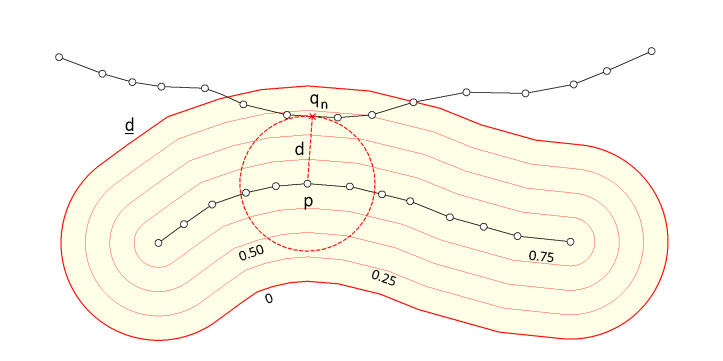
\includegraphics[width=11cm]{images/spline.png} 
    \caption{Energetická funkce $E_e(x,y)$ se znázorněnými vrstevnicemi (převzato z Bayer 2023).}
\end{figure}
\par Energetická funkce pro tuto operaci má tvar
\begin{equation*}
E_e(x, y) = \begin{cases}
    c(1-\frac{d}{\underline{\textit{d}}}), \quad d < \underline{\textit{d}}\\
    0, \quad \quad \qquad \text{jinak},\\
    \end{cases}
\end{equation*}
\par kde $c$ je konstanta, $c \in \mathbb{R}^+$, a ovlivňuje míru, jakou tento člen upravuje tvar splinu. V diskrétní podobě využívá řešení parciálních derivací $E_e$ podle $x, y$:

\begin{equation*}\begin{split}
    \frac{\partial E_e(x,y)}{\partial x} &= -c \frac{x - x_n}{d \underline{\textit{d}}}, & \qquad
    \frac{\partial E_e(x,y)}{\partial y} &= -c \frac{y - y_n}{d \underline{\textit{d}}},
\end{split}
\end{equation*}

kde $q_n = [x_n, y_n]$ je nejbližší vrchol k vrcholu $p = [x, y]$. Výsledné posuny vrcholů vycházejí z požadavku vyrovnaného stavu mezi vnitřní a vnější energií.

\subsection*{Částečná modifikace jednoho prvku}
\par Tato varianta se v kartografii využívá v případě, kdy chceme, aby svůj tvar a polohu modifikoval pouze generalizovaný prvek. Tento případ může nastat například ve vztahu silniční sítě a vodstva, kde by vodní tok měl představovat nehybný prvek a neměl by být generalizací dotčen. 
\par Algoritmus pro tuto variantu operace Partial Modification je složen z následujících kroků:
\begin{enumerate}
    \item  Předzpracování: konverze spojové reprezentace polylinie na maticovou reprezentaci.
    \item Výpočet kroku $h$.
    \item Určení prvků matice $A$ ze zadaných hodnot $\alpha, \beta, \gamma$ a $h$.
    \item Iterační proces: postupné realizování posunu pro předem zadaný počet iterací, výpočet nových souřadnic vrcholů splinu.
    \item Konverze maticové reprezentace $X, Y$ na spojový seznam vrcholů generalizované polylinie.
\end{enumerate}